\documentclass[a4, 12pt]{scrreprt}

\usepackage{amsmath}
\usepackage[T1]{fontenc}
\usepackage[utf8]{inputenc}
\usepackage{enumitem}
\setlist[itemize]{nosep,after=\vskip-\baselineskip,leftmargin=*,before=\minipagetrue,}

\makeatletter
\newcommand{\minipagetrue}{\@minipagetrue}

\makeatother
\usepackage{graphicx}
\usepackage[T1]{fontenc}
\usepackage[ngerman]{babel}
\usepackage[colorlinks,
pdfpagelabels,
pdfstartview = FitH,
bookmarksopen = true,
bookmarksnumbered = true,
linkcolor = black,
plainpages = false,
hypertexnames = false,
citecolor = black] {hyperref}

\setcounter{secnumdepth}{1}
\setcounter{tocdepth}{1}

\begin{document}

\tableofcontents



\part{Überblick Gesteine}

\chapter{Magmatite}

\begin{itemize}
\item Erstarrungsgesteine
\item meist aus Silikatschmelzen entstanden
\item seltener Karbonat-, Sulfid- und Phosphatschmelzen
\end{itemize}

\section{Plutonite}

\begin{itemize}
\item Intrusivgestein (Tiefengestein)
\item entstehen aus langsam abkühlenden Magmen, welche in der Erdkruste in andere Gesteine eingedrungen sind
\item $\rightarrow$ langsame Erstarrung \begin{itemize}
\item wenige Kristallkeime, langes Keimwachstum
\item große Kristalle, kein Glas
\end{itemize}
\end{itemize}

\section{Vulkanite}
\begin{itemize}
\item Eruptiv-, Effusivgestein (Ergussgestein)
\item bilden sich aus Schmelzen, welche bei Eruptionen an die Oberfläche gelangen
\item $\rightarrow$ schnelle Abkühlung
\begin{itemize}
\item schnelle Erstarrung
\item viele Kristallkeime, wenig Kristallachstum
\item viele kleine Kristalle, oft auch Glasbildung
\end{itemize}
\end{itemize}

\chapter{Sedimente und Sedimentgesteine}

\section{Bildung}

Kriterien:
\begin{itemize}
\item  Gefüge häufig lagig-schichtig oder massig, bei Tonen auch feinschichtig
\item Korngröße variiert zwischen sehr fein und grob – auch in einem Gestein
\item bei grobkörnigen Sedimenten lassen sich Mineral- und Gesteinstrümmer und das
die Trümmer verkittende Bindemittel (Matrix / Zement) bestimmen
	\begin{itemize}
	\item alle Minerale und Gesteinsarten können als Fragmente vorhanden sein
	\item kristallines Bindemittel ist meist durch chemische Prozesse entstanden
	\item teilweise sind Fossilien erkennbar oder das Sediment besteht fast ausschließlich aus Fossilien
	\end{itemize}
\item häufig porös (z.T. sehr feingliedrig), aber auch dicht
\item mitunter nicht verfestigt (keine Ausschlusskriterium! $\rightarrow$ vgl. Pyroklasika)
\end{itemize}

Ausgangsgesteine sind Magmatite, Plutonite oder Prä- existente Sedimentgesteine\\

Prozess:
\begin{enumerate}
\item Verwitterung
	\begin{itemize}
	\item an der Erdoberfläche
	\item Zerkleinerung es Ausgangsmaterials durch exogene Kräfte in 			verschieden große Partikel/Fragmente bzw. Lösungen
	\item physikalische/chemische/biogene Verwitterung
	\end{itemize}
\item Erosion und Transport
	\begin{itemize}
	\item Seen, Flüsse, Meer
	\item Eis (Gletscher)
	\item Wind (z.B in Wüsten)
	\item Mensch und Tier (Biogen)
	\item Schwerkraft (Abbruch von Klippen
	\end{itemize}
\item Sedimentation
	\begin{itemize}
	\item sobalt die Tragkraft nicht mehr für den Transport ausreicht
	\item Bildung von Lockersedimenten
	\end{itemize}
\item Diagenese
	\begin{itemize}
	\item chemische und/oder Physikalische Vorgänge die zur Umbildung eines lockeren Sediments zu einem verfestigten Sediment führen\\
	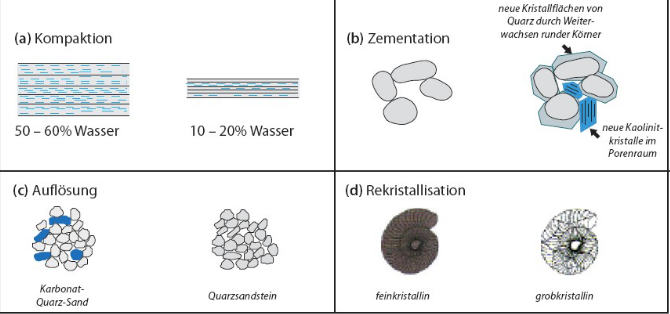
\includegraphics[width=0.8\textwidth]{/home/joni/Schreibtisch/Uni/Mittschriften/Bausteine Der Erde/Bilder/Sedimentbildung.png}
	\item Wesentliche FAktoren bei der Sedimentbildung:
		\begin{itemize}
		\item Druck (lithostatischer Druck und Porenfluiddruck)
		\item Temperatur (geotherm. Gradient, Mächtigkeit Überdeckung, Magmatismus)
		\item Zeit (Dauer der Einwirkung)
		\item Mineralogie des Ausgangs-Sediments (chem./physikal. Stabilität, reaktive Oberfläche)
		\item Struktur und Gefüge des Ausgangs-Sediments (Korngröße, Sortierung, Porosität)
		\item Zusammensetzung der Porenlösungen (pH, chemische Zusammensetzung)
		\item sedimentäres und tektonisches Milieu (Mächtigkeit der Sedimente, Porenwasserstrom)
		\end{itemize}
	\end{itemize}
\end{enumerate}

\section{klastische Sedimente}

Trümmergesteine\\
überwiegend mechanische Anhäufung von Gesteinsfragmenten und Einzelkörnern\\
Produkt von überwiegend mechanischer Verwitterung\\
z.B Konglomerat oder Sandstein

\section{chemische Sedimente}

aus Lösungen ausgefällt (teilweise mit klastischem Anteil)\\
z.B. Salzgesteine

\section{biogene Sedimente}

vorwiegend aus organischem Material entstanden (teilweise mit klastischem Anteil)
z.B. Riffkalk oder Kohle

\section{Farbe von Sedimentgesteinen}

Abhängig von:\\
\begin{tabular}{ll}
rot & Hämatit ($Fe_2O_3$); mit abnehmender Korngröße zunehmende Intensität\\
grün & Glaukonit, chlorit, Illit\\
schwarz/grau & organische Restsubstanz\\
gelbbraun & Geothit (FeOOH)
\end{tabular}

\section{wichtige Minerale in Sedimentgesteinen}
\begin{itemize}
\item Quarz
\item Plagioklase, Feldspäte
\item Muskovit, Biotit, Tonminerale, Chlorit
\item Pyroxene, Amphibole
\item Calzit, Dolomit
\item Gips, Anhydrit, Steinsalz, Kalisalz
\item Pyrit
\end{itemize}

\part{Gesteinsbestimmung von Sedimenten}

\chapter{Äußerliche Merkmale}

\section{Farbe}
rot, grün, schwarz, grau, gelbbraun, etc.

\section{Gesteinsform}
locker oder fest

\section{Bruch(-flächen)}
unregelmäßig; wenige, viele, etc.

\chapter{Gemengeteile}
Siehe Chapter \ref{sec:Gemengeteile}

\chapter{Struktur}

\section{Kristallinität}
kristallin, nicht kristallin / klastisch, Matrix, Mineralneubildung?

\section{relative Korngröße}

gleichkörnig oder ungleichkörnig
\begin{tabular}{ll}
konglomerat & abgerundete Gesteinsbruchstücke\\
Brekzie & kantige Gesteinsbruchstücke\\
\end{tabular}

\section{Absolute Korngröße}

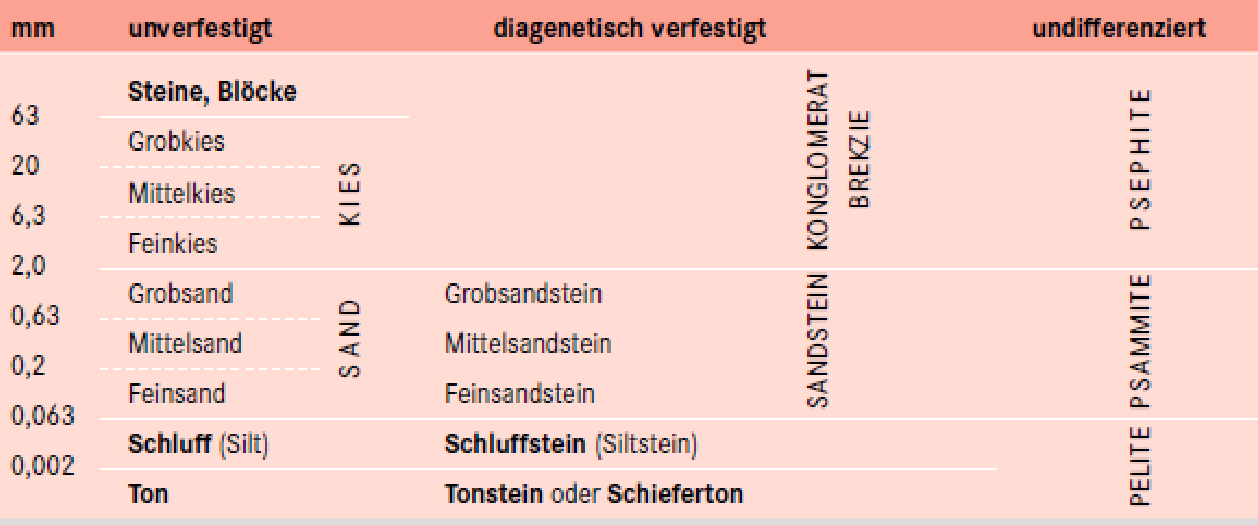
\includegraphics[width=0.8\textwidth]{/home/joni/Schreibtisch/Uni/Mittschriften/Bausteine Der Erde/Bilder/Sedimentunterteilung.png}

\section{Kornform, Rundungsgrad, Oberflächen}
\begin{tabular}{l|l}
Rundungsgrad & 
	\begin{tabular}{l}
	kugelförmig\\
	eiförmig\\
	diskusförmig\\
	plattig\\
	stengelig\\
	\end{tabular}\\
	
Kornoberflächen & 
	\begin{tabular}{l}
	glatt\\
	narbig\\
	geritzt\\
	\end{tabular}\\

Rundungsgrad \\
\end{tabular}\\
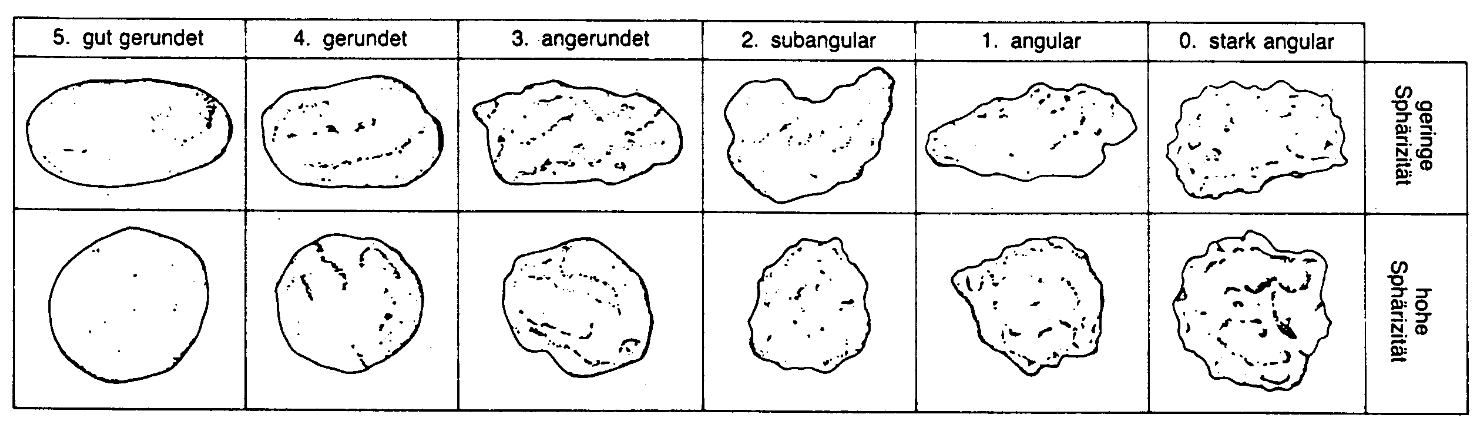
\includegraphics[width=0.8\textwidth]{/home/joni/Schreibtisch/Uni/Mittschriften/Bausteine Der Erde/Bilder/Rundungsgrad.png}\\

\section{Sortierungsgrad, Kornverband}
gut bzw. schlecht sortiert

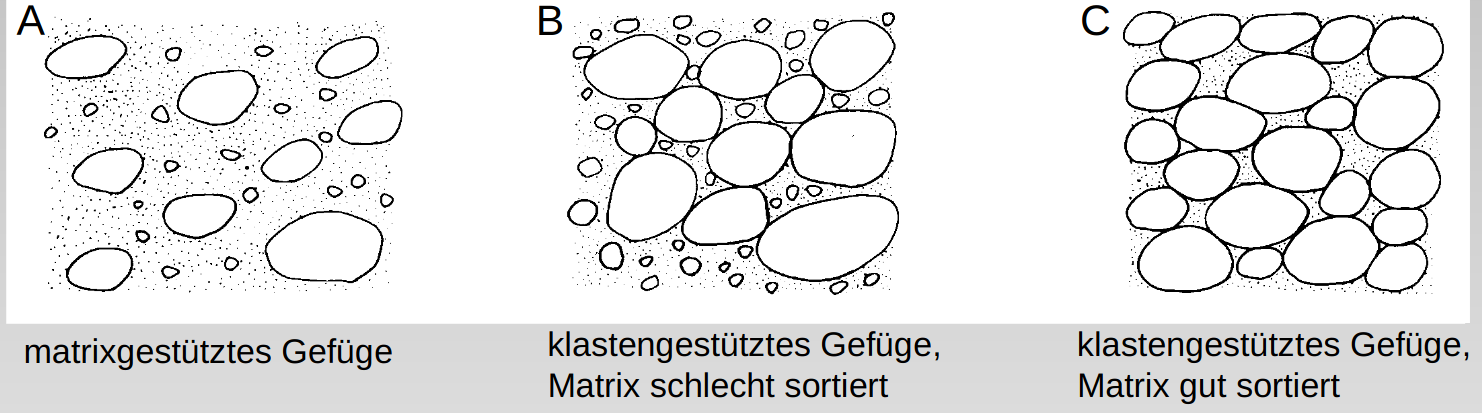
\includegraphics[width=0.8\textwidth]{/home/joni/Schreibtisch/Uni/Mittschriften/Bausteine Der Erde/Bilder/Kornverband_Sediment.png}\\

\section{Bindemittel}

\begin{tabular}{p{3cm}@{}p{9cm}@{}}
Zement & 
	\begin{itemize}
	\item Material, das die Kornkomponenten eines Sedimentes "verkittet"
	\item 
		\begin{tabular}{p{3cm}@{}p{6cm}@{}}
		diagenetisch ausgefällt & Tone und chemische Ausfällungsprodukte, die im Raum zwischen den einzelnen Körnern (Intergranularraum) eines (Locker)Sedimentes nach dessen Ablagerung gebildet wurden, d.h. authigen (am selben Ort)\\
		\end{tabular}
	\item z.B. kieselig; tonig; karbonatisch; eisenschüssig
	\end{itemize}\\
	
Matrix & 
	\begin{itemize}
	\item fein zerriebener Detritus
	\item gleichzeitig mit sedimenten abgelagert (aber andernorts gebildet)
	\item z.B. tonig, siltig, sandig; monomikt/polymikt; karbonatisch (mikrokristallin)
	\end{itemize}\\
\end{tabular}



\section{Reife}

\begin{tabular}{p{3cm}@{}p{9cm}@{}}
mechanisch & 
	\begin{itemize}
	\item reif: gleichkörnig
	\item unreif: ungleichkörnig
	\end{itemize}\\
chemisch &
	\begin{itemize}
	\item reif: chemisch homogen
	\item unreif: chemisch heterogen
	\end{itemize}
\end{tabular}\\


\part{Gesteinsbestimmung von Magmatiten}

\chapter{äußerliche Merkmale}

\section{Farbe}

\begin{itemize}
\item Grad der Verwitterung
\item Farbe der gesteinsbildenen Minerale
\item Größe der Minerale und Gesteinskomponenten
\item Menge und Oxidationsgrad des vorhandenden Eisens 
\item Menge und Art des organischen Materials
\item Feuchtigkeit des Gesteins
\end{itemize}

\section{Gesteinsform/Größe}
Größe, ggf. Geometrische abmaße/Form

\section{Bruch/Spaltbarkeit}
\begin{itemize}
\item muschelig: kreisförmige Reifen an der Bruchhstelle, z.B. Glas
\item uneben: keine Regelmäßigkeit der Bruchkannten, z.B Sylvin
\item erdig: glanzlos und stumpf, z.B Aluminit
\item glatt: Baryt
\item faserig: gleicht kleinen Hährchen, z.B Gips
\item splittrig: Absonderung kleiner Splitter
\item hakig: kleine scharfe wiederhaken z.B Eisen
\end{itemize}

\section{Bruchflächen}
\begin{itemize}
\item regellos, gerundet, gerade, Parallel zum Gefüge
\item glatt, ungleichmäßig, rau
\item Kanten gerundet/scharf/splittrig
\item Ausbrüche von (herausstehenden) Komponenten
\item frisch/verwittert
\end{itemize}

\newpage
\chapter{Gemengeteile} \label{sec:Gemengeteile}

\section{Matrix}
Farbe, prozentualer Anteil, Körnigkeit etc.

\section{Mineralbeschreibung}

\subsection{Farbe/Strichfarbe}

Farbe des Minerals

\subsection{Glanz}

\begin{itemize}
\item Diamantglanz
\item Fettglanz
\item Glasglanz
\item Matter Glanz
\item Metallglanz
\end{itemize}

\subsection{Transparenz}

\begin{itemize}
\item durchsichtig
\item durchscheinend
\item kantendurchscheinend
\item durchsichtig
\end{itemize}

\subsection{Härte}
\begin{tabular}{lll}
Härte & Beispiel & wird geritzt von\\
\hline
1 & Talk\\
2 & Gips & Fingernagel\\
3 & Kalzit\\
4 & Fluorit & Edelstahl und ungehärteter Stahl\\
5 & Apatit & gehärteter Stahl\\
6 & Kalifeldspat & Fensterglas\\
7 & Quartz\\
8 & Topas\\
9 & Korund\\
10 & Diamand\\
\end{tabular}

\subsection{Bruch}
uneben, spröde, splittrig

\subsection{Spaltbarkeit}

$\rightarrow$ ebener Bruch\\

Grad:
\begin{itemize}
\item vollkommen
\item gut
\item deutlich
\item schlecht
\end{itemize}

Orientierung:
\begin{itemize}
\item 45
\item 60
\item 90
\item 120
\end{itemize}

\subsection{Verzwillingung}

\begin{itemize}
\item Karlsbader Zwilling (bei Alkalifeldspäten)
\begin{itemize}
\item Kristalle gleicher Zusammensetzung verwachsen
\item Hälften refletieren in verschiedene Richtungen
\end{itemize}
\item Polysynthetische Verzwillingung (bei Plagioklasen)
\begin{itemize}
\item eng anenander
\item parallel
\item keine Eigenfarbe
\end{itemize}
\end{itemize}

\subsection{Habitus/Wuchsform}

\begin{itemize}
\item isometrisch
\item lang/kurzprismatisch
\item rhomboedrisch
\item (di)-pyramidal
\item nadelig
\item faserig
\item blättrig
\item etc.
\end{itemize}

\subsection{Magnetismus}

ja/nein

\subsection{Dichte}

vereinzelt/eher gebunden/in Gruppen

\section{Gesteinsbruchstücke}

vorhanden oder nicht?

\chapter{Struktur}

\section{Korngröße}

\begin{itemize}
\item makrokristallin: Minerale mit bloßem Auge erkennbar
\item mikrokristallin: Minerale mit der Lupe erkennbar
\item kryptokristallin: Mineral unter dem Mikroskop erkennbar
\end{itemize}

\section{Korngröße}

\begin{center}
\begin{tabular}{lc}
Bezeichnung & Korndurchmesser in mm\\
\hline
riesenkörnig & >30\\
großkörnig & 10-30\\
grobkörnig & 3-10\\
mittelkörnig & 1-3\\
kleinkörnig & 0,3-1\\
feinkörnig & 0,1-0,3\\
dicht & <0,1\\
\end{tabular}
\end{center}

\section{Korngrößenverteilung}
\textbf{Korngrößenverteilung:}\\
äquigranular: gleichkörnig\\
heterogranular: wechselkörnig

\section{Korngrößenvergleich}

\begin{itemize}
\item gleichkörnig
\begin{itemize}
\item gleichkörnig grob-,mittel-,feinkörnig
\end{itemize}
\item ungleichkörnig
\begin{itemize}
\item Sedimente: konglomeratisch/brekziös
\item Vulkanite: porphyrisch
\item Plutonite: porphyrartig
\item Metamorphite: Porphyroblastisch
\end{itemize}
\end{itemize}

\section{Grad der Kristallinität}
\begin{center}
\begin{tabular}{ll}
holokristallin & vollständig kristallisiert\\
hypokristallin & nicht vollständig kristallisiert\\
hyalin & glasig/nicht kristalliert\\
\end{tabular}
\end{center}

\section{Kornform}

\begin{center}
\begin{tabular}{ll}
idiomorph & eigengestaltig\\
hypidiomoph & z.T. eigengestaltig\\
xenomorph & fremdgestaltig
\end{tabular}
\end{center}

\section{Kornbindung}

\begin{itemize}
\item unmittlbare Kornbindung
\begin{itemize}
\item einzelkristalle grenzen unmittelbar aneinander
\item Zusammenhalt des Gesteins durch Grenzflächenkräfte, enge Verzahnung der Einzelkörner
\end{itemize}
mittelbare Kornbindung
\begin{itemize}
\item Einzelbestandteile des Gesteins durch Bindemittel (Zement) verkittet
\item vor Allem bei Sedimenten
\end{itemize}
\end{itemize}

\chapter{Textur}

\section{Art der Raumfüllung}

\begin{itemize}
\item kompakt
\item blasig
\item schaumig
\item zellenartig
\item porös
\end{itemize}

\section{räumliche Verteilung der Gefügeelemente}

\begin{center}
\begin{tabular}{ll}
homogen & gleichmäßig\\
inhomogen & ungleichmäßig\\
\end{tabular}
\end{center}

\section{Räumliche Orientierung der Gefügeelemente}

\begin{center}
\begin{tabular}{@{}lp{9cm}@{}}
isotop & richtungs-, regellos\\
anisotop & \begin{itemize}
\item richtungsabhängige Orientierung Paralleltextur
\item Material oder Korngrößenwechsel (inhomogener Verteilung der Einzelelemente)
\end{itemize}\\
\end{tabular}
\end{center}

\chapter{Bestimmung}

\section{Magmatische Gesteine}

\subsection{<90\% Anteil mafischen Gesteins}

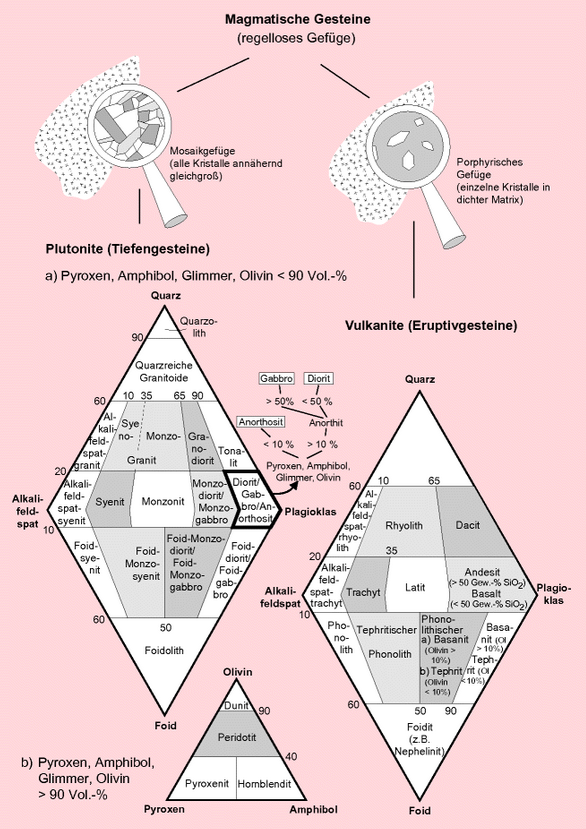
\includegraphics[width=0.7\textwidth]{/home/joni/Schreibtisch/Uni/Mittschriften/Bausteine Der Erde/Bilder/BestimmungsDrachenviereck.png}

\subsubsection{Plagioklasbestimmung}

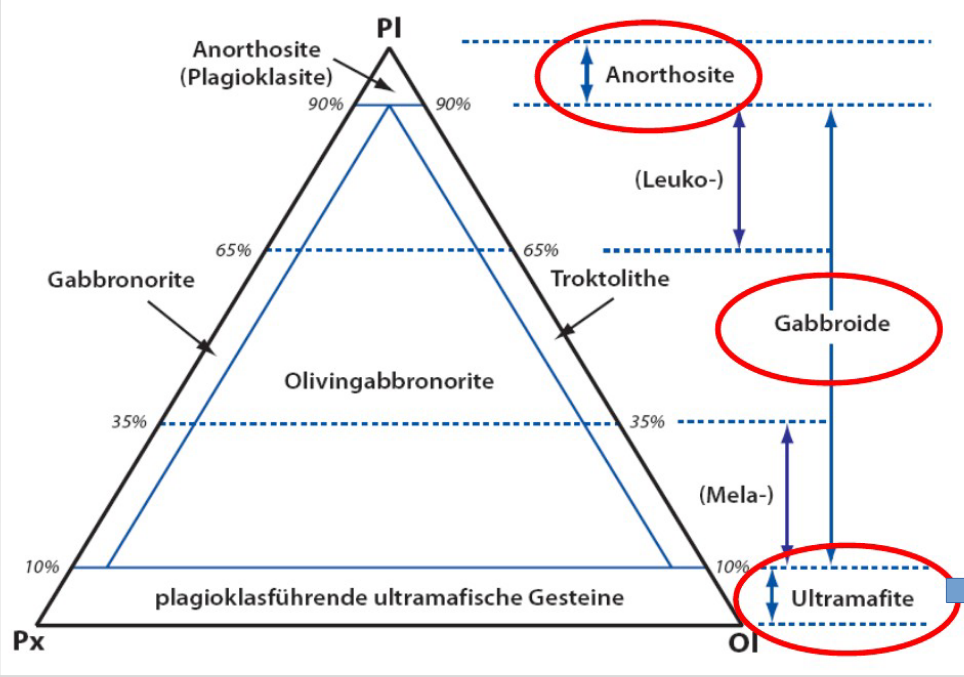
\includegraphics[width=0.8\textwidth]{/home/joni/Schreibtisch/Uni/Mittschriften/Bausteine Der Erde/Bilder/Plagioklasbenennung.png}

\subsection{mit >90\% Anteil mafischen Gesteins}

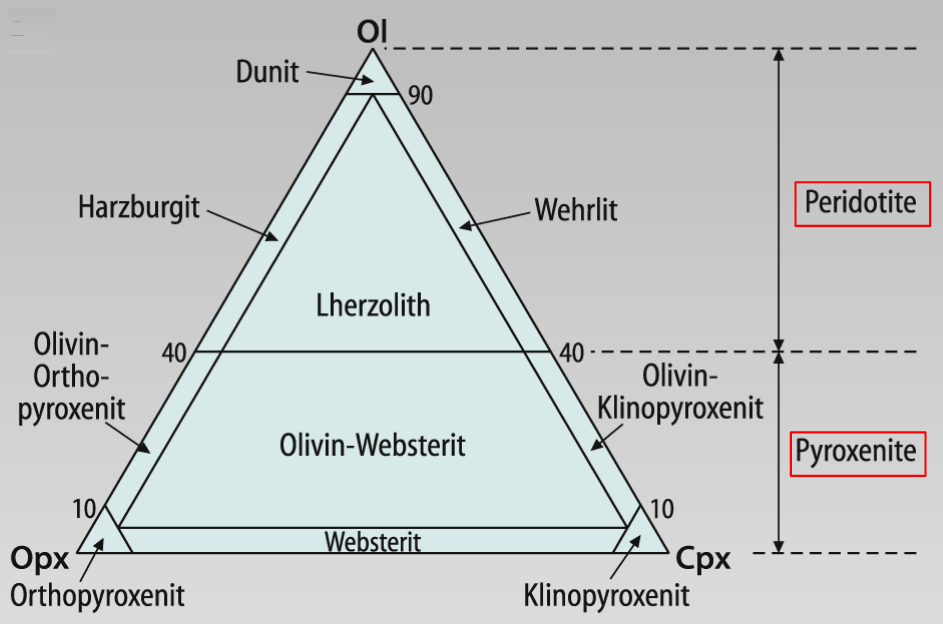
\includegraphics[width=0.8\textwidth]{/home/joni/Schreibtisch/Uni/Mittschriften/Bausteine Der Erde/Bilder/ultramafische_Benennung.png}


\part{Wörterbuch}

\chapter{Definitionen}

\begin{tabular}{p{5cm}@{}|p{11cm}@{}}
\hline
Mineral & chemisch homogener, natürlich vorkommender Festkörper, meist kristallin und anorganisch. \\
\\
 & \begin{tabular}{@{}l|p{9cm}@{}}

homogen & einheitliche physikalische/chemische Eigenschaften, kann auch durch mechanische Verfahren nicht weiter in seine Bestandteile zersetzt werden.\\
\\
natürlich & ohne Einfluss des Menschen entstehend\\
\\
Festkörper & weder flüssig noch gasförmig (Ausnahme Quecksilber)\\
\hline
\end{tabular}\\
\hline
Kristall & Festkörper, deren Atome dreidimensional periodisch geordnet sind dh. eine geordnete in alle drei Raumrichtungen wiederhohlende struktur bilden. \\
\hline
Gestein & Natürlich vorkommende Mineralvergesellschaftung deren Zusammensetztung und Gefüge innerhalb eines Volumens gleichförmig ist.\\
\hline
Paragenese/\\Mineralvergesellschaftung & unterschiedliche Minerale kommen in dierektem Kornkontakt in einem Gestein vor, doch die Identität der einzelnen Minerale wird beibehalten\\
\hline
Pseudomorphose & Verdrängung oder Ersatzt von Stoffen, wobei die Form erhalten bleibt sich aber die Chemie ändert\\
\hline
Benennung von Gesteinen nach mafischem Anteil & 
\begin{tabular}{p{3cm}@{}p{6cm}@{}}
leukokrat & 0-35\%\\
mesotyp & 35-65\%\\
melanokrat & 65-90\%\\
ultramafisch & >90\%\\
\end{tabular}\\
\hline

Pyroklastische Gesteine & 
\begin{tabular}{p{3cm}@{}p{6cm}@{}}
lockere Pyroklastite & Tephra\\
verfestigte Pyroklastite & vulkanische Tuffe; bestehen aus Aschekörnern, Lapili oder Blöcken/Bomben\\
\\
 \begin{tabular}{l|lp{4,5cm}@{}}
 Fragmentgröße & lockere Pyroklastite & verfestigte Pyroklastite\\
 >64mm & Bomben/Blöcke & Blocktuff (polyklastische Breccie)\\
 2 bis 64mm & Lapili & Lapilituff (Lapilistein)\\
 <2mm & Asche & Aschentuff \\
 \end{tabular}\\
\end{tabular}\\
\hline
\end{tabular}






\end{document}